In this chapter we introduce Bayesian inference and multilevel modelling. We then explore how to fit and evaluate Bayesian models.

\section{Introduction}

Bayes theorem, and by extension Bayesian statistics and inference, is named after an amateur mathematician and Presbyterian minister from the 18th century, the Reverend Thomas Bayes. After Bayes' death, his friend Richard Price found an essay Bayes wrote titled ``an imperfect solution of one of the most difficult problems in the doctrine of chances''. Price saw the value in Bayes' work and submitted it to the Royal Society for publication. In Bayes' time (circa the 17-18th centuries) probability and statistical theory as we know it today was in its infancy and not widely studied as it is now. The leading probability thinkers of the time conceived of the subject through the lens of gambling and games of chance \cite{David1998} \cite{Moivre1718}. The thinkers of the time had reasoned about probability from cause to effect in these contexts (e.g. what are the odds of getting four aces in a poker hand?). What Bayes had shown in his essay was a potential solution to a yet unsolved problem: the so-called inverse-probability problem of reasoning from effect to cause (e.g. if a player deals himself four aces in three hands in a row, what are the odds his deck is loaded?). The legendary mathematician Pierre Simone Laplace fused Bayes' ideas with his own and published what we now know as Bayes theorem in 1825 \cite{Stigler1986}. The legacy of Bayes and Laplace's work is that we now refer to the general approach of using data (effect) to estimate parameters (cause) through the use of Bayes' theorem as Bayesian statistics and inference.

Bayes theorem can be stated simply as:
\begin{equation} \label{eq:orig_bayes_theorem}
P(A|B) = \frac{P(B|A)P(A)}{P(B)}
\end{equation}
This equation can be derived from basic rules of probability and conditional probability, namely that $P(A \cap B) = P(A|B)P(B)$ and equivalently $P(A \cap B) = P(B|A)P(A)$. One can then simply substitute and isolate $P(A|B)$ to arrive at equation \ref{eq:orig_bayes_theorem}.

Bayes theorem is usually derived from the basic rules of probability and introduced as equation \ref{eq:orig_bayes_theorem}, and then counter-intuitive examples are used to show the efficacy of the theorem (e.g. a test for a rare disease is 99\% accurate, if you test positive what is the probability that you have the disease?). However, Bayesian statistics extends \ref{eq:orig_bayes_theorem} to the context of data and model parameters. In this extension, Bayes theorem instead describes a joint probability distribution over all observed and unobserved parameters in a statistical model \cite{Schoot2021}. With a data set $x$ and parameters $\theta$, we can rewrite Bayes theorem as:

\begin{equation} \label{eq:new_bayes_theorem}
P(\theta|x) = \frac{P(x|\theta)P(\theta)}{P(x)}
\end{equation}

In equation \ref{eq:new_bayes_theorem}, each part of the equation is referred to and interpreted differently than in \ref{eq:orig_bayes_theorem}. The conditional probability $P(\theta|x)$ is referred to as the \textit{posterior} distribution and represents the probability of the model parameters, $\theta$, conditional on the data, $x$. The conditional probability of the data given the model parameters, $P(x|\theta)$, is referred to as the \textit{likelihood}. The probability of particular model parameter values existing in the population, $p(\theta)$, is referred to as the \textit{prior} distribution. The denominator, $p(x)$, functions as merely a normalizing factor to ensure that the posterior probabilities sum to $1$, but it does not change their relative values. Notice that $p(x)$ does not explicitly depend on $\theta$. Thus, we can simplify \ref{eq:new_bayes_theorem} by dropping $p(x)$ and re-interpret Bayes theorem recognizing that the posterior distribution is proportional to the likelihood function multiplied by the prior distribution:

\begin{equation} \label{eq:proportional_bayes_theorem}
P(\theta|x) \propto P(x|\theta)P(\theta)
\end{equation}

Intuitively, Bayesian statistics starts with a prior belief (i.e. prior distribution over parameters of a model) and then updates that belief with new information (i.e. the likelihood of the data) resulting in an updated posterior belief (i.e. the posterior distribution of model parameters). This updated posterior will then serve as the new prior distribution when more information is available in the future for us to yet again update our belief. In this way our beliefs are continually updated with data in order to make them increasingly more accurate. While this intuition is generally appealing on its own, more importantly Bayesian statistics has been successful in solving challenging problems in applied statistics both historically and more recently \cite{Schoot2021}. Despite its intuitive appeal and real world successes, Bayesian statistics actually declined in popularity during the first half of the 20th century. Understanding this decline and how it has been overcome shows why Bayesian techniques are becoming increasingly popular in the modern scientific era.

The primary reasons for the decline in the popularity of Bayesian statistics were an objection to the ``subjective'' use of prior distributions, and the difficulty in actually computing the posterior distribution in \ref{eq:new_bayes_theorem}. Most prominent statisticians of the early 20th century did not like the ``subjectivity'' of specifying a prior that could potentially influence the results of inference for what was supposed to be objective science. In particular, many of the most prominent statisticians of the 20th century, including R.A. Fischer and Karl Pearson, were vocal opponents of subjectivity and Bayesian statistics which they saw as being synonymous. This ``smear campaign'' combined with computational difficulties led much of statistics and science to turn to judging the probability of an event according to how frequently it occurs among many observations. This preferred view of statistics, lauded by its theorists of the early 20th century as being ``objective'', led to the widespread adoption of traditional statistical methods often referred to as \textit{frequentist} statistics. Despite these challenges, Bayesian statistics still saw some use and success in real-world contexts including but not limited to actuarial science and military applications \cite{McGrayne2011}. Meanwhile traditional frequentist methods have come under increasing criticism in recent decades \cite{Ioannidis2005} \cite{Begley2015}. Scientists in the modern era are becoming increasingly aware that all statistical methods are subjective in the sense that all statistical techniques make assumptions. Bayesian statistics is merely more transparent about its assumptions in its model formulation than most other methods. While subjectivity in the form of using priors was originally seen as a negative, it is instead now seen as a strength. Since ``all models are wrong, but some are useful'' \cite{Box1976}, it is more responsible to be upfront and clear about the subjective assumptions of any statistical model or methodology rather than blindly optimizing a misunderstood technique, such as seeking a p-value $<$ 0.05.

The second primary reason for the decline of Bayesian statistics in the 20th century is the difficulty in actually computing \ref{eq:new_bayes_theorem} for most problems. The computational difficulties arise specifically from the normalization factor $(P(x))$ in \ref{eq:new_bayes_theorem}. The normalization factor can also be thought of as the probability of the dataset, which is something we generally don't know a priori. Thus, we have to turn to the law of total probability in order to compute it which means that the calculation of this normalization factor requires integrating over all possible parameters $(\theta)$ as follows:

\begin{equation} \label{eq:normalization_factor}
P(x) = \int_{\theta} P(x|\theta)P(\theta) d\theta
\end{equation}

The integral in \ref{eq:normalization_factor} can sometimes be computed in low dimensions, most often in situations known as \textit{conjugate priors} where the prior and likelihood conveniently combine into another known distribution. However, in higher dimensions where the number of parameters making up $\theta$ is larger and when using distributions for the prior and likelihood that do not form convenient conjugate pairings, the integral in \ref{eq:normalization_factor} becomes mathematically intractable. This means the integral can not be computed exactly and instead can at best be approximated using numerical techniques. However, many of the numerical techniques and computing devices we have today did not exist in the first half of the 20th century which meant Bayesian methods were out of reach for most scientists. The advances in computing as well as the theory behind numerical techniques, most notably Markov Chain Monte Carlo, have made approximating the posterior in \ref{eq:new_bayes_theorem} computationally feasible which has greatly contributed to the resurgence of Bayesian techniques in recent decades.

\section{Multilevel Modelling} \label{Multilevel_Modelling}

The process of having a prior belief, updating it with new information, and then taking the resulting posterior to be your updated belief, or your new prior belief moving forward, is a process that often resonates with people and how their views and beliefs about the world are constructed and updated. While not only intuitively appealing, there are also many practical examples where the use of a prior distribution in Bayesian inference leads to better results \cite{Schoot2021}. This makes Bayesian inference an appealing option; however, actually constructing or deciding on a prior distribution can be difficult. Multilevel modelling is a method that sets up the prior distribution to be learned from the data. This makes specifying a prior easier as the data is primarily determining the prior, and it generally also leads to better out-of-sample predictive performance, making multilevel modelling an attractive option. This section provides background to understand how multilevel modelling works and describes the motivation for using multilevel modelling. The effectiveness of multilevel modelling is further explored in the data experiments described in the Methods chapter.

Multilevel modelling can be viewed as a trade-off between two extremes: \textit{complete-pooling} and \textit{no-pooling}. Complete-pooling is when an overall average is used and variations among groups or categories within the overall data are ignored, thus the data are ``completely pooled''. No-pooling is when separate models for each individual group or category are used and any correlations or dependencies among the groups are ignored, thus the data is ``not pooled'' at all. In this view, multilevel models are seen as \textit{partially-pooled} where their estimates can be thought of as a trade-off between the complete-pooling (e.g. overall group mean) and no-pooling (e.g. individual group means) extremes. For groups with fewer data points the multilevel model produces estimates more similar to the complete-pooling estimate, and for groups with more data points the model produces estimates more similar to the no-pooling estimates. This results in what is commonly referred to as \textit{shrinkage} whereby partially pooled estimates are essentially the no-pooling estimates that have been “shrunk” toward to complete-pooling estimate, or ``shrunk toward the mean''. The amount of shrinkage depends on the samples-sizes, the variation within groups, and the variation between groups.

It is helpful to consider an estimate from a simple partially pooled model in order to understand how partial-pooling works. Consider a model that has one categorical predictor indicating which group an observation belongs to (e.g. which province a voter lives in), and no other predictors. In this case the partially pooled model will generate predictions for each group by constructing a weighted average of the group level means and the overall mean. Mathematically it would be constructed like this:

\begin{equation} \label{eq:mlm_ex}
\hat{\alpha}_j^{multilevel} \approx \frac{ \frac{n_j}{\sigma_y^2} \bar{y}_j + \frac{1}{\sigma_{\alpha}^2} \bar{y}_{all} }{ \frac{n_j}{\sigma_y^2} + \frac{1}{\sigma_{\alpha}^2} }
\end{equation}

\begin{figure}
	\centering
	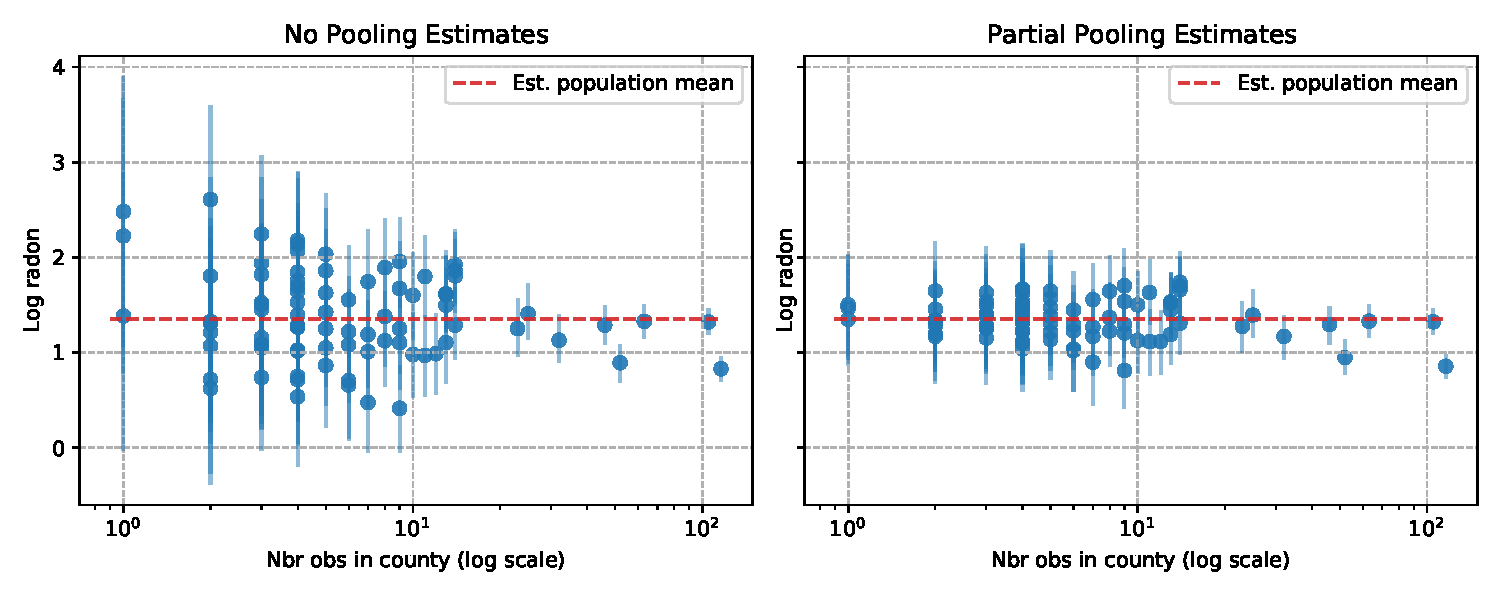
\includegraphics[width=\textwidth]{figures/radon_example.pdf}
	\caption{Comparison of county parameter estimates between traditional regression (no pooling) and multilevel regression (partial pooling). Notice how the partial pooling estimates ``shrink toward the mean''. Further note how this shrinkage is greater for the counties with fewer observations and lesser for counties with more observations.}
	\label{fig:radon_example}
\end{figure}

where $\hat{\alpha}_j^{multilevel}$ is the estimate from the multilevel model for the j-th group. It is the weighted average of the j-th groups average ($\bar{y}_j$) and the average of all groups combined ($\bar{y}_{all}$). The weights are determined by the within-group variance ($\sigma_y^2$), the sample size of the j-th group ($n_j$), and the variance among the groups ($\sigma_{\alpha}^2$). In this way, larger (smaller) sample sizes for the j-th group and the lower (greater) within-group variance leads to larger (smaller) weight placed on the j-th group average for the final estimate. Smaller (larger) variance among the groups leads to a larger (smaller) weight placed on the overall average for the estimate of the j-th group. This view makes it clear that the estimates from a multilevel model will compute a group estimate in a similar way to a more traditional regression model but will then shrink that estimate toward the overall mean weighted by the groups sample size, the within group variance, and the among group variances. Here the overall mean and how much the estimates should shrink toward it is determined by the data and represents the prior distribution over the parameters which is then conditioned by the data. It is in this manner that the prior is learned from the data by pooling information across groups.

Equation \ref{eq:mlm_ex} has an $\approx$ symbol rather than an $=$ symbol because it is only in a few mathematically convenient cases, such as conjugate priors, that the group level estimate would precisely reduce to the formula in equation \ref{eq:mlm_ex}. Including more predictors, more mathematically complex transformations and other engineered features, and using more varied probability distributions that do not result in conjugate priors, all lead to estimates that are no longer mathematically tractable and instead require approximation methods such as Markov chain Monte Carlo to generate the estimates. However, even in such complex cases where the estimates cannot be computed analytically they still in practice function the same way as outlined by equation \ref{eq:mlm_ex} \cite{Gelman2006}.

For a more concrete example of the regularizing shrinkage to the mean effect of multilevel modelling we consider the canonical example from Andrew Gelman's work \cite{Gelman2006} \cite{Gelman2006b}, which is now often considered as the introductory tutorial of multilevel modelling \cite{pymc32018}. In \cite{Gelman2006b} the strengths and limitations of multilevel modelling are illustrated through an example of the prediction of home radon levels in U.S. counties. To identify areas of high radon exposure, the Environmental Protection Agency coordinated the collection of radon measurements in a random sample of more than 80,000 houses in the United States. In addition to these measurements were predictors for indicating if the measurement was on the first floor of the home or in the basement, and what the county uranium levels are for each county in which the homes were located (approximately 3000 counties total). Gelman showed that multilevel modelling outperformed traditional regression modelling as measured by out-of-sample performance estimated by cross-validation prediction errors.

A simplified example of the work in \cite{Gelman2006b} is shown in Figure \ref{fig:radon_example} where we compare the results of fitting a traditional regression model and a multilevel regression model that estimates house radon levels using the county that the houses belong to as the only predictor for the counties in the state of Minnesota. This simplified model can be expressed as $y_i = \alpha_{j[i]} + \epsilon_i$, where $y_i$ is the radon level for house $i$ ($i=1, \cdots ,919$), $\alpha_{j[i]}$ is the average radon level for the j-th county ($j=1, \cdots ,85$) of which the i-th house belongs, and $\epsilon_i$ represents the random errors due to measurement error, temporal within-house variation, or variation among houses. As previously discussed, the traditional regression model will model radon in each county independently resulting in no-pooling estimates, while the multilevel model will pool information across counties to make estimates similar to equation \ref{eq:mlm_ex} resulting in partial-pooling estimates. We note how the counties with fewer observations result in greater shrinkage towards the overall mean, while counties with more observations stay closer to their no-pooling estimates. The overall mean across counties acts as a regularizing prior distribution, but this prior was also learned from the data. This regularizing effect of shrinking individual group parameter estimates towards the overall group mean is the essential idea behind multilevel modelling. The advantages of multilevel modelling are thoroughly explored in the works of \cite{Gelman2014} \cite{Gelman2006} \cite{McElreath2020} and are summarized here to provide further motivation for the use of multilevel modelling in this thesis.

Multilevel modelling is useful because it can be viewed as a ``white-box'' method whereby each part of the model can be fully interpreted, understood, and customized. This makes it ideal for inference. Furthermore, multilevel models are Bayesian graphs which means that Judea Pearl’s causal calculus (or ``do-calculus'') can be used to infer causality \cite{Pearl2000}. This makes multilevel models useful beyond predictions alone. In contrast, many machine learning methods such as neural networks and ensemble decision trees are not interpretable.

Many datasets have an inherent multilevel structure for which multilevel modelling can provide more efficient inference of regression parameters (e.g. students within schools, patients within hospitals, laboratory assays on plates, elections in districts within states, or data from cluster sampling etc.). Even ``simple'' cross-sectional data can be placed in a larger multilevel context. For example, many datasets initially thought to be ``big data'' often become ``small data'' once you begin sub-dividing them into more and more sub-groups. For example, opinion polls trying to predict who voters will vote for based on age, race, income, location, interests etc. Each split leaves smaller and smaller groupings that have the potential for better model fit, since there are more predictors, at the risk of over-fitting, since sample sizes of the sub-groups become increasingly small.

Multilevel models allow for including predictors at two different levels of a regression model. You can specify models that have individual level predictors and group level predictors. For example, in estimating radon levels in houses you could have measurements at the individual level (individual houses, indicator if the sensor is in the basement, etc.) and then predictors at the group level (county-level uranium readings) and using both together provides better model fit than separating them \cite{Gelman2006b}.

Multilevel modelling avoids problems in classical regression such as collinearity when trying to include group-level indicators as well as group-level predictors in the same model by using \textit{index variables} instead of \textit{dummy variables}. This is most noticeable when considering the ``reference group'' that results from using dummy variables to encode categorical variables in traditional regression. $N$ many categories can be encoded with $N-1$ many dummy variables. For example, consider three categories only requiring two dummy variables we can refer to as $\alpha$ and $\beta$. The first category is encoded with $\alpha = 1$ and $\beta = 0$. The second category is encoded with $\alpha = 0$ and $\beta = 1$. The third category is encoded with $\alpha = 0$ and $\beta = 0$; there is no need for a third dummy variable. If a third dummy variable is added the resulting system of equations used to solve for the coefficients for each indicator variable becomes singular \cite{Fox2008}, which means you cannot get estimates for the regression coefficients using linear algebra. Furthermore, because the third category is encoded by the absence of the first two, it does not get its own regression coefficient and instead the intercept and all other regression coefficients of the model are changed to reflect this. As a result, the intercept will now represent the third category and the coefficients for the other categories will represent differences relative to the third category. This makes the third category the reference group and can be a source of confusion when interpreting a model. In Bayesian modelling this requires specifying a prior distribution for the difference of each category from the reference category, as well as a prior distribution for the reference category. By contrast, an index variable gives an index to each category (a unique integer for each category, starting at 1 and increasing up to the number of categories) and does not require a reference group. This allows for assigning the same prior distribution to each category, which cannot be done with dummy variables, and makes scaling a model to include more or new categories seamless. It also makes interpreting the coefficients for each category easier as they no longer represent differences from one of the categories. Leveraging index variables allows multilevel models to avoid issues with collinearity while being more interpretable.

Multilevel modelling aids in inferring the right standard error by accurately accounting for uncertainty in prediction and estimation. To get an accurate measure of predictive uncertainty, one must account for correlation of the outcome between groups, categories, and predictors (e.g. forecasting state-by-state outcomes in the U.S. election, one must account for correlation of outcome between states in a given year). This becomes more useful in cases where the uncertainty in estimation is of interest rather than the estimate itself.

Sometimes predictions require multilevel modelling, such as when making predictions for a new group. For example, consider a model of test scores for students within schools. You could model school-level variability in classical regression (or another machine learning model such as decision trees or neural nets) with an indicator for each school. But it is impossible in this framework to make a prediction for a new student in a new school, because there is no indicator in the model for this new school. This type of problem is handled seamlessly when using the multilevel framework by using group level predictors to estimate where the new school would fall relative to the other groups.

Multilevel modelling is attractive because it comes with all the benefits of regression modelling while generally outperforming classical regression modelling in predictive accuracy. The primary source of improvement over classical regression is due to the shrinkage of parameter estimates generally improving out-of-sample predictive fit. The improved performance is due to using all the data to perform inferences for groups, especially those with small sample sizes. At one extreme classical estimation can be useless if the sample size is small in a group or category. At the other extreme classical regression ignores group-level variation which can be misleading especially when some groups have small sample sizes. Multilevel modelling compromises between the overall noisy within-group estimates (no-pooling) and the oversimplified regression estimate that ignores group variation (complete-pooling). The shrinkage effect of multilevel modelling acts as a form of regularization that protects from over-fitting to produce more accurate predictions on unseen data. Over-fitting in regression modelling and how multilevel models help prevent it is explored further in the first data experiment described in \ref{experiment_1}.

While the benefits of multilevel modelling are bountiful, they are mathematically more complex than classical regression and are generally mathematically intractable. This means we can not compute the parameter estimates directly and instead need to approximate them with more advanced numerical approximation techniques.

\section{Markov chain Monte Carlo}

\begin{figure}
	\subfloat[]{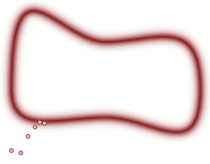
\includegraphics[width=0.5\textwidth]{figures/finding_typical_set.png}} 
	\subfloat[]{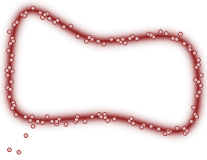
\includegraphics[width=0.5\textwidth]{figures/exploring_typical_set.png}} \\
	\subfloat[]{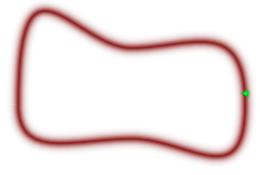
\includegraphics[width=0.5\textwidth]{figures/mcmc_typical_set.png}} 
	\subfloat[]{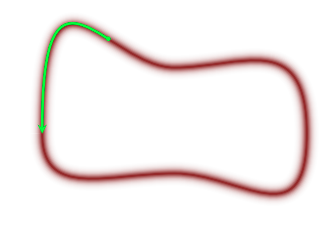
\includegraphics[width=0.5\textwidth]{figures/hmc_typical_set.png}}
	\caption{Under ideal circumstances a Markov chain will first converge to the typical set (a) and then explore it efficiently (b). Unfortunately, in higher dimensions most MCMC algorithms struggle to explore the typical set and inefficiently sample a small portion (c, green). We desire algorithms that make use of the geometry of the target distribution to properly explore the typical set during sampling (d). Images are from Figures 7, 10, 11 of \cite{Betancourt2017}. Permission to use was granted by the author under a CC BY-NC 4.0 license (https://creativecommons.org/licenses/by-nc/4.0/).}
	\label{fig:mcmc}
\end{figure}

For most models of practical interest, exact inference is intractable, and so we have to resort to some form of approximation \cite{Bishop2006}. The primary end goal of Bayesian inference is computing the posterior distribution. It is with the posterior distribution that we can perform inference and answer questions about quantities of interest. The issue is that computing the posterior distribution for nearly all but the simplest of models is not only difficult but often impossible. That is to say that we can not derive a closed form mathematical expression that represents the posterior distribution. We can, however, approximate the posterior. Researchers have developed many different methods of numerical approximation which can be employed to approximate the posterior distribution in Bayesian inference.

Most methods that attempt to approximate the posterior distribution (or approximate integrals more generally) work well in low-dimensional settings but struggle or outright fail in high-dimensional settings due to a phenomenon known as \textit{concentration of measure}. Concentration of measure refers to the fact that in low dimensions the probability mass of a distribution is concentrated around its mode, but in higher dimensions the probability mass of a distribution is surprisingly not concentrated around its mode and becomes increasingly further away from the mode as the dimensionality increases. The probability mass of a distribution concentrates into a density band into which almost all random draws from a distribution will fall, and is referred to as the \textit{typical set}. The typical set is therefore precisely where we want to sample from in order to generate accurate approximations of the posterior distribution. For a deeper treatment of these concepts see \cite{Betancourt2017} \cite{Carpenter2017}. The models considered in this thesis are relatively high-dimensional, therefore we employ the current state of the art, Hamiltonian Monte Carlo (HMC), for approximating high-dimensional posterior distributions by sampling efficiently from the typical set. In order to understand what makes HMC so effective we first explore its simpler foundational method, Markov chain Monte Carlo (MCMC).

The most common method to approximate computing a desired probabilistic quantity is to repeatedly draw independent samples from the probability distribution and to then average over those samples to approximate the quantity of interest. This is known as Monte Carlo sampling.  Just as statisticians traditionally aim to draw independent samples in order to estimate desired quantities, such as the mean, variance, or specific quantiles, about a target population, Monte Carlo sampling aims to draw independent samples from a probability distribution in order to approximate the distribution or a specific property of that distribution.

Drawing independent samples from a known distribution to then only be able to approximate said distribution appears counter-intuitive at best and wholly wasteful at worst. In practice, however, we do not actually know the distribution that we want to sample from. The most powerful and surprising insight of statistical computing, and MCMC in particular, is that we can sample from a distribution that we do not know and then use those samples to approximate the unknown distribution. We can do this by drawing samples from, or ``visiting'' each part of, the distribution in proportion to its relative probability. Sampling in proportion to the relative probability of a distribution is done by making Markov transitions via the use of a Markov chain. We then draw samples in this manner enough times to generate a sequence of samples that closely approximates the distribution of interest.

A Markov chain is a probabilistic model that describes a sequence of possible states in which the probability of each state depends only on the previous state. This means that no matter how the process arrived at the current state, the possible future states are fixed based on the current state. This allows you to go from one state to another repeatedly as many times as you desire or need to. The entire sequence of states you visit then represents a chain. For our purposes, we can think of states as locations in the parameter space of the distribution which we are trying to sample from, and the chain is the sequence of samples. Future states can then be determined by the relative probability density of other locations in the parameter space, computed as in \ref{eq:proportional_bayes_theorem}. This forms the basis of one of the most well-known MCMC algorithms, the Metropolis algorithm.

The simplest and most well known MCMC algorithm, the Metropolis algorithm, begins by randomly selecting a starting location in the parameter space, generates a new ``proposal'' location to move to in the parameter space, but only moves to this new location if it has a higher density relative to the previous location or by random chance proportional to the difference in relative densities of the current location to the proposed location. As the algorithm runs for more samples, it will visit each location in the parameter space proportional to the probability density of each location, thus the sequence of samples will approximate the probability distribution more accurately as more samples are drawn. The drawback of this algorithm is trying to determine how many samples is enough. While it has been shown that the samples will tend toward the correct proportions and thus correct probability densities \cite{Metropolis1953} \cite{Hastings1970}, there is no rigorous general theory to determine how many samples is enough and how accurate your approximation actually is so that you can know if you have sampled enough.

There have been many advances upon and extensions of the Metropolis algorithm that attempt to improve the generalizability and efficiency of the sampling. These include but are not limited to the Metropolis-Hastings algorithm and Gibbs sampling \cite{Hastings1970} \cite{German1984}. These algorithms can broadly be grouped together as ``guess and check'' algorithms. They ``guess'' a random proposal of where to move, they then ``check'' the posterior probability at that location and compare it to the current location. The consequence is that the quality of proposals becomes the primary bottleneck. If the algorithm makes poor proposals then much of the compute time of the algorithm is wasted when it could be touring the parameter space collecting more samples instead of rejecting proposals.

Many of the extensions of the Metropolis algorithm do try to overcome this by having a tunable step-size parameter. While it does help in some cases, this step-size parameter leads to a trade-off between improving the acceptance rate of proposals at the cost of exploring the parameter space and vice versa. A smaller step-size will improve the acceptance rate of proposals and will lead to more samples being accepted and thus more efficient sampling; however, this comes at the cost of not being able to explore or tour the full parameter space as efficiently and thus more samples are needed to get a representative sample of the parameter space. These small steps from one proposal to the next will often result in the samples staying in the same area and often ``re-exploring'' the same areas opposed to exploring the full parameter space. Increasing the step-size will improve the exploration but will come at the cost of a lower acceptance rate of proposals as proposals will more often be from low probability areas of the distribution. Furthermore, as the dimensionality of the parameter space increases so too does the concentration of measure which only exacerbates the challenge of efficiently exploring the parameter space of the typical set for these algorithms. Figure \ref{fig:mcmc} illustrates the idealized scenario for MCMC algorithms.

The fundamental issue with guess and check algorithms is that proposals are generally bad when they are random and don't know anything about the target distribution. This issue is further exacerbated when trying to estimate distributions that have high-dimensional parameter spaces, because of the previously mentioned phenomenon concentration of measure \cite{Betancourt2017} \cite{Carpenter2017}. This makes the random proposals from ``guess and check'' methods increasingly inefficient and ultimately poor estimators of distributions with many parameters. To overcome this researchers have turned to creating algorithms that try to incorporate more information from the target distribution when making proposals in order to explore the typical set more efficiently. The current state of the art is known as Hamiltonian Monte Carlo and is the method employed in this thesis to fit Bayesian models.

\section{Hamiltonian Monte Carlo}

\begin{figure}
	\subfloat[]{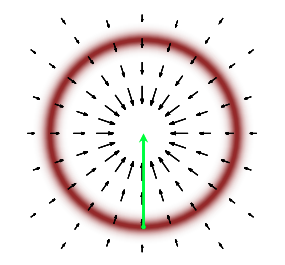
\includegraphics[width=0.5\textwidth]{figures/gradient_prob_system.png}} 
	\subfloat[]{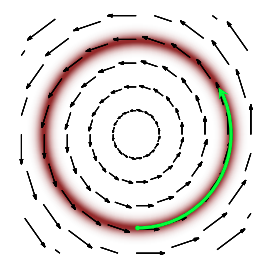
\includegraphics[width=0.5\textwidth]{figures/gradient_adj_prob_system.png}} \\
	\subfloat[]{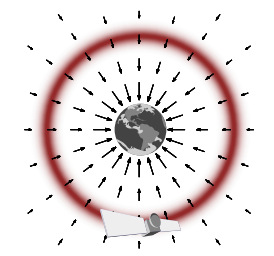
\includegraphics[width=0.5\textwidth]{figures/gradient_phys_system.png}} 
	\subfloat[]{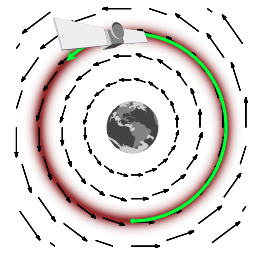
\includegraphics[width=0.5\textwidth]{figures/gradient_adj_phys_system.png}}
	\caption{The gradient and corresponding vector field of a probability distribution points to its mode which is often away from the typical set in higher dimensions (a). Ideally we want to twist the vector field to align with the typical set (b). The mode, gradient, and typical set of a probabilistic system are mathematically equivalent to a planet, gravitational field, and orbit in a physical system (c). Adding momentum to the system to cause a satellite to enter a stable orbit (d) is equivalent to twisting a vector field to align with the typical set of a probabilistic system. Images are from Figures 12, 13, 14, 17 of \cite{Betancourt2017}. Permission to use was granted by the author under a CC BY-NC 4.0 license (https://creativecommons.org/licenses/by-nc/4.0/).}
	\label{fig:hmc}
\end{figure}

Hamiltonian Monte Carlo (HMC) exploits information about the geometry of the typical set to greatly improve the efficiency at accurately sampling the paramter space of the target distribution. The insight of HMC is that for every probabilistic system there is a mathematically equivalent \textit{physical} system, with equivalent differential geometry, about which we can reason and solve for in the exact same way a physicist would compute the conservative dynamics of a physical system via phase space and Hamilton's equations \cite{Betancourt2017}; hence the name Hamiltonian Monte Carlo.

HMC works by exploiting the \textit{gradient} of the target probability density function, defines a vector field that we can manipulate to be aligned with the typical set. Then we can follow this vector field in order to explore and sample from the typical set more efficiently. By itself, the gradient of the target probability density function points towards the mode of the distribution, and thus away from the typical set. Additional structure is required to twist the vector field generated by the gradient into a vector field aligned with the typical set. This additional structure can be thought of as adding \textit{momentum} in such a way as to keep the corresponding dynamics of the system \textit{conservative}. That is to say that the conservative dynamics of the physical system requires volumes to be preserved in accordance with Hamilton's equations. A rigorous derivation and exposition of conservative dynamics and Hamilton's equations is beyond the scope of this thesis but can be found in \cite{Betancourt2017}. Here we give an intuitive explanation of how conservative dynamics in physical systems works and how it relates to the probabilistic systems considered in this thesis. The intuitive relation between a probabilistic system and a physical system is illustrated in Figure \ref{fig:hmc}.

Intuitively, a mode, a gradient, and a typical set in a probabilistic system can be equivalently related to a planet, a gravitational field, and an orbit in a physical system. Exploring this physical system with a satellite is mathematically equivalent to exploring and sampling our probabilistic system. A satellite at rest will fall to the planet due to the planets gravitational pull. Adding momentum to the satellite allows it to enter a stable orbit and not be pulled into the planet. However, adding too much momentum causes the satellite to leave the stable orbit and fly out to the depths of space. Conversely, adding too little momentum causes the satellite to again be pulled into the planet. Adding just the right amount of momentum to the satellite for it to remain in a stable orbit is the mathematical equivalent of the corresponding dynamics of the system remaining conservative, and is computed by ensuring the preservation of volume in position-momentum phase space \cite{Betancourt2017}. For our purposes, the above analogy means that the same mathematics used to compute how much momentum to add to a physical system in order to ensure the corresponding dynamics are conservative (i.e. putting a satellite into a stable orbit) can be used to twist the gradient of a target probability density function and its vector field into one that corresponds to the typical set. We can then make proposals by taking steps proportionally random to the vector field that follows the typical set. This will ensure that our sample proposals will be attracted toward the typical set, and will then stay in and efficiently explore the typical set.

For this thesis we make use of the Probabilistic Programming library PyMC3 \cite{pymc3} and its implementation of HMC to fit our models. PyMC3 and our use of it to build and fit our models is explored more in the Methods chapter.

\section{Model Evaluation and Selection}

It is not enough to simply create a model and fit it to a dataset. There are infinitely many models that could be created and fit to a dataset, and some models will be better than others depending on the context or objective of the model. Thus, it is important we evaluate how well a given model fits a dataset and gauge its predictive performance. This allows us to understand how effectively a given model fits our dataset and it gives us a way to select the ``best'' model from among several models.

Model selection in a Bayesian context separates itself from more traditional null hypothesis testing by considering the existence of many possible models rather than assuming one model and evaluating its likelihood. Null hypothesis testing has a single (null) model and seeks data such that the model can be judged as sufficiently likely or unlikely. In contrast, Bayesian model selection assumes that there exists many potential models that could have generated the dataset we have, and instead tries to reason about which of those models was more likely to have produced the dataset. Thus we need tools to compare models in order to select the ``best fitting'' one, or the one that was most likely to have produced the data. This section describes how we evaluate the efficacy of Bayesian models via cross validation, information theory, and posterior predictive checks.

\subsection*{Cross Validation, Information Criterion, and Beyond}
It is natural to desire a model that fits the dataset as well as possible. However, it is possible to create models that fit a specific dataset so well that they fail to generalize to the larger population of which the dataset is only a sample. When this happens we say that a model is ``over-fit''. While fitting a given dataset as well as possible seems desirable, it often comes at the cost of the model only fitting and retrodicting the dataset it was trained on and then performing much worse on unseen data or future scenarios for which the model was ideally created for. Thus it is important that we do not evaluate a model only on the basis of how well it fits and retrodicts the dataset it was trained on, but that we try to estimate how well the model fits the larger population and its ability to predict unseen data that it was not trained on.

Because a models performance on unseen data is more desirable than its performance on the data it was trained on, researchers have developed methods that actually make a model fit worse to the data it was trained on so that it fits unseen data better. This counter-intuitive idea is known as \textit{regularization} and is a vast area of research in statistical inference and machine learning. Bayesian models perform regularization through the use of priors and through a process in multilevel modelling known as shrinkage to the mean which has previously been discussed in section \ref{Multilevel_Modelling}. In order to see the effect of regularization and to compare various models we need a method of model evaluation. This section explores how we evaluate models through estimating their evaluation on unseen data.

\begin{figure}
	\subfloat[]{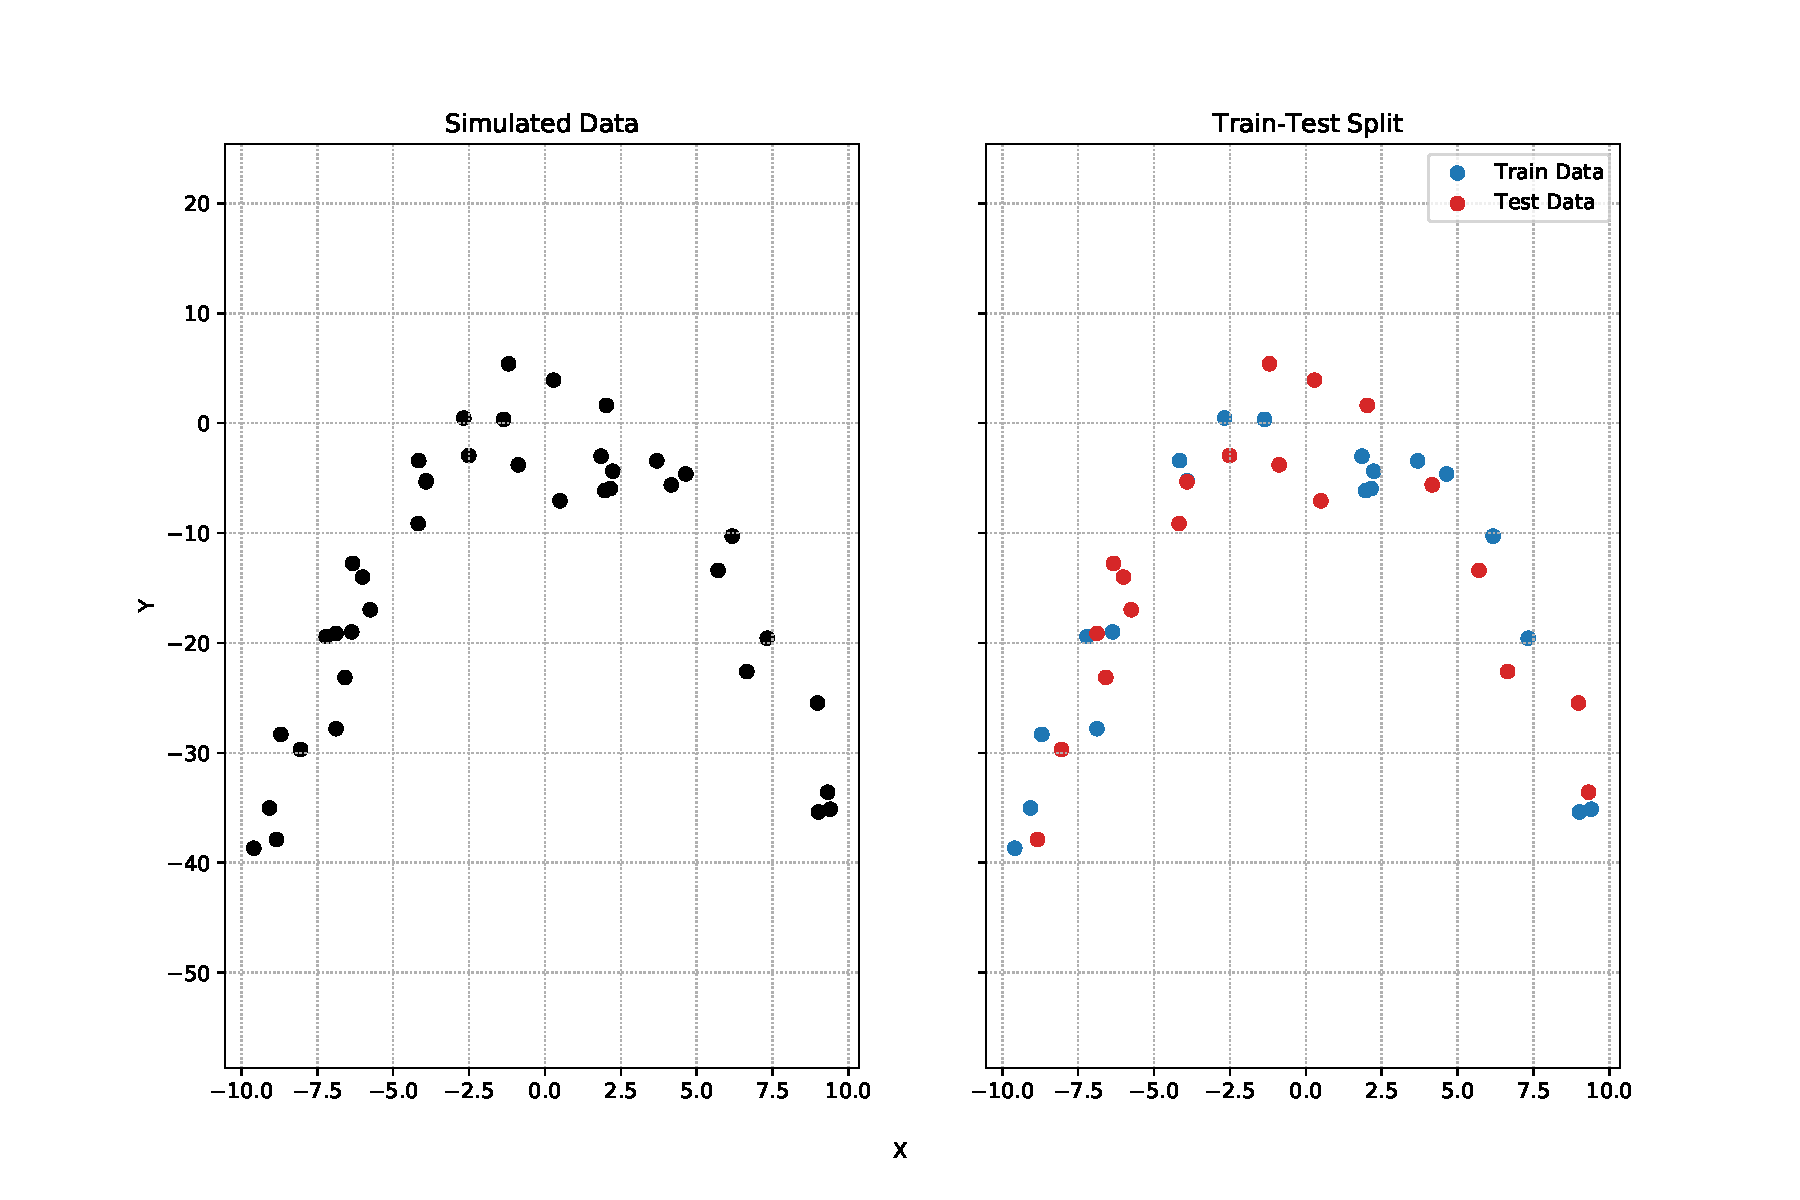
\includegraphics[width=0.5\textwidth]{figures/generated_data_and_splits.pdf}} 
	\subfloat[]{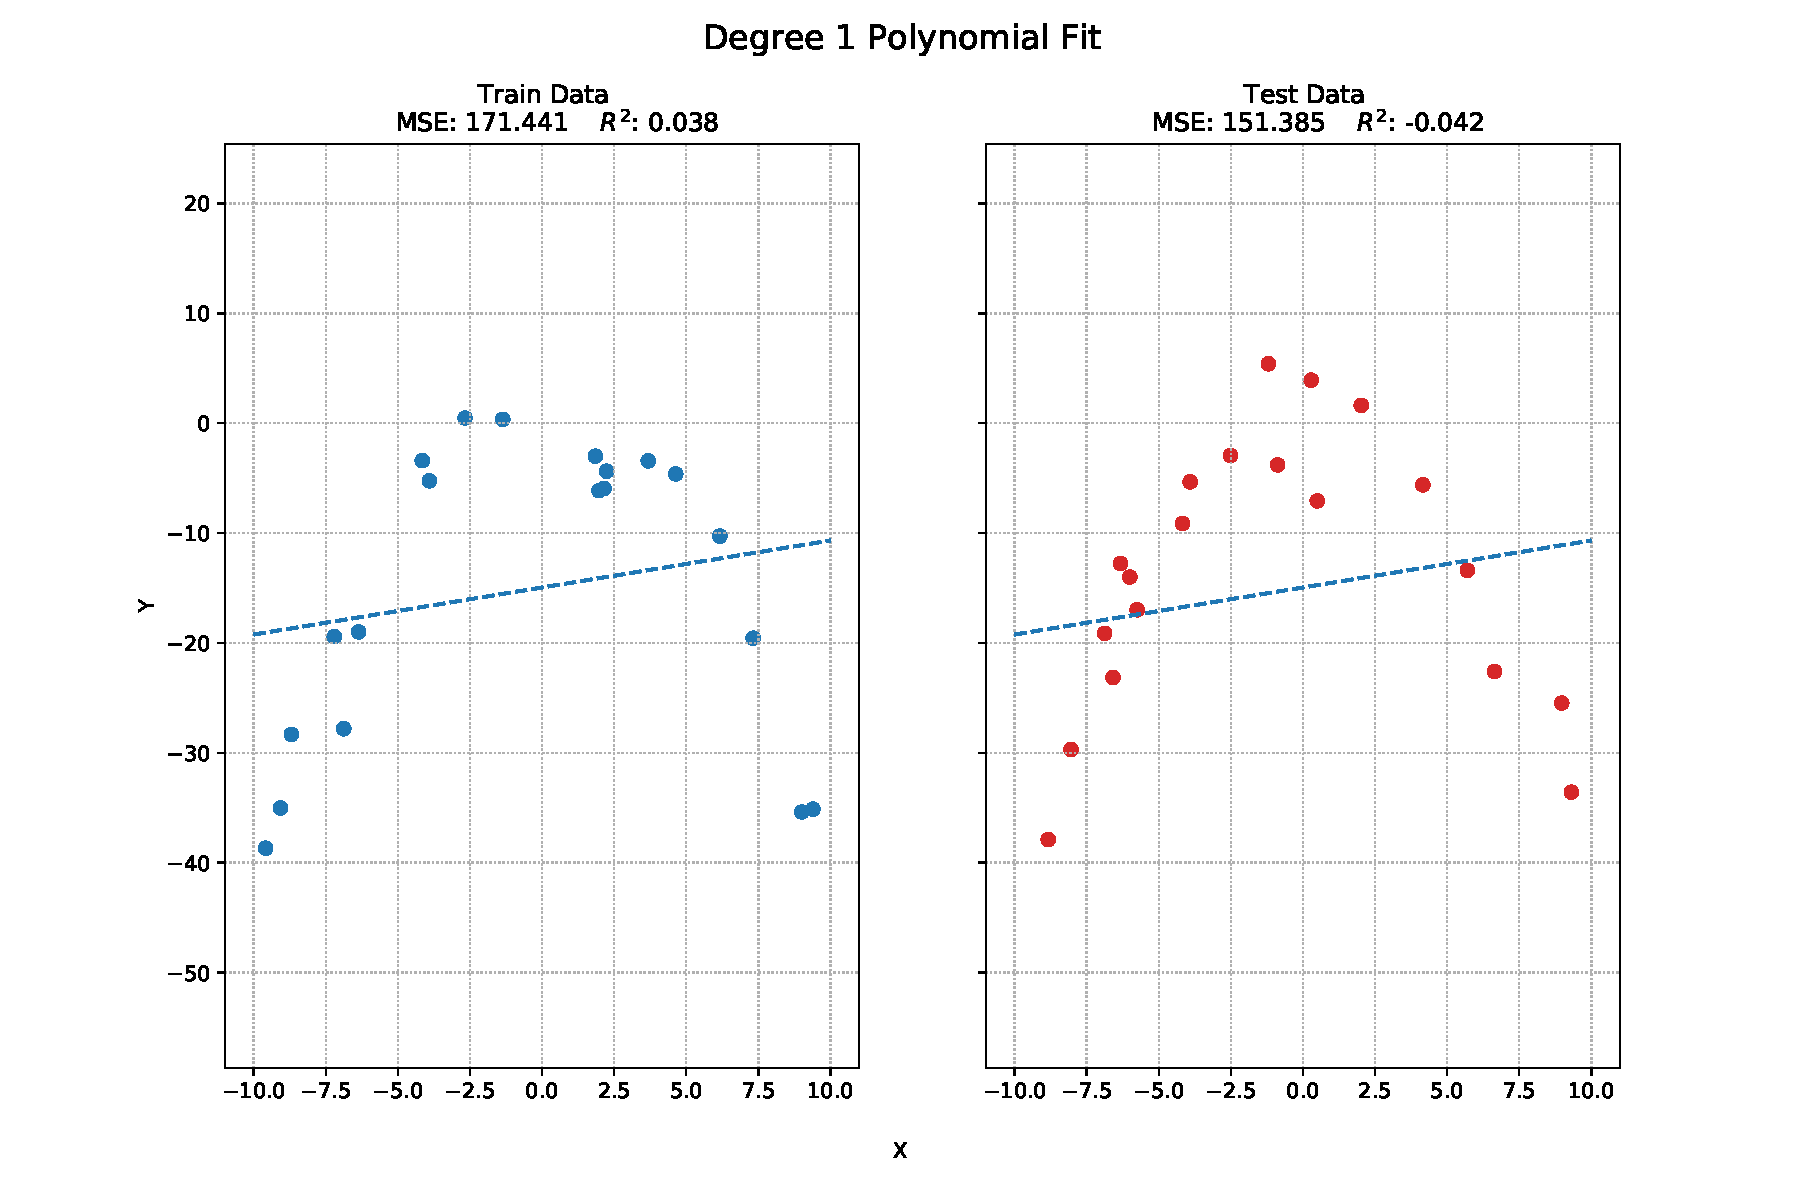
\includegraphics[width=0.5\textwidth]{figures/poly_fit_1.pdf}} \\
	\subfloat[]{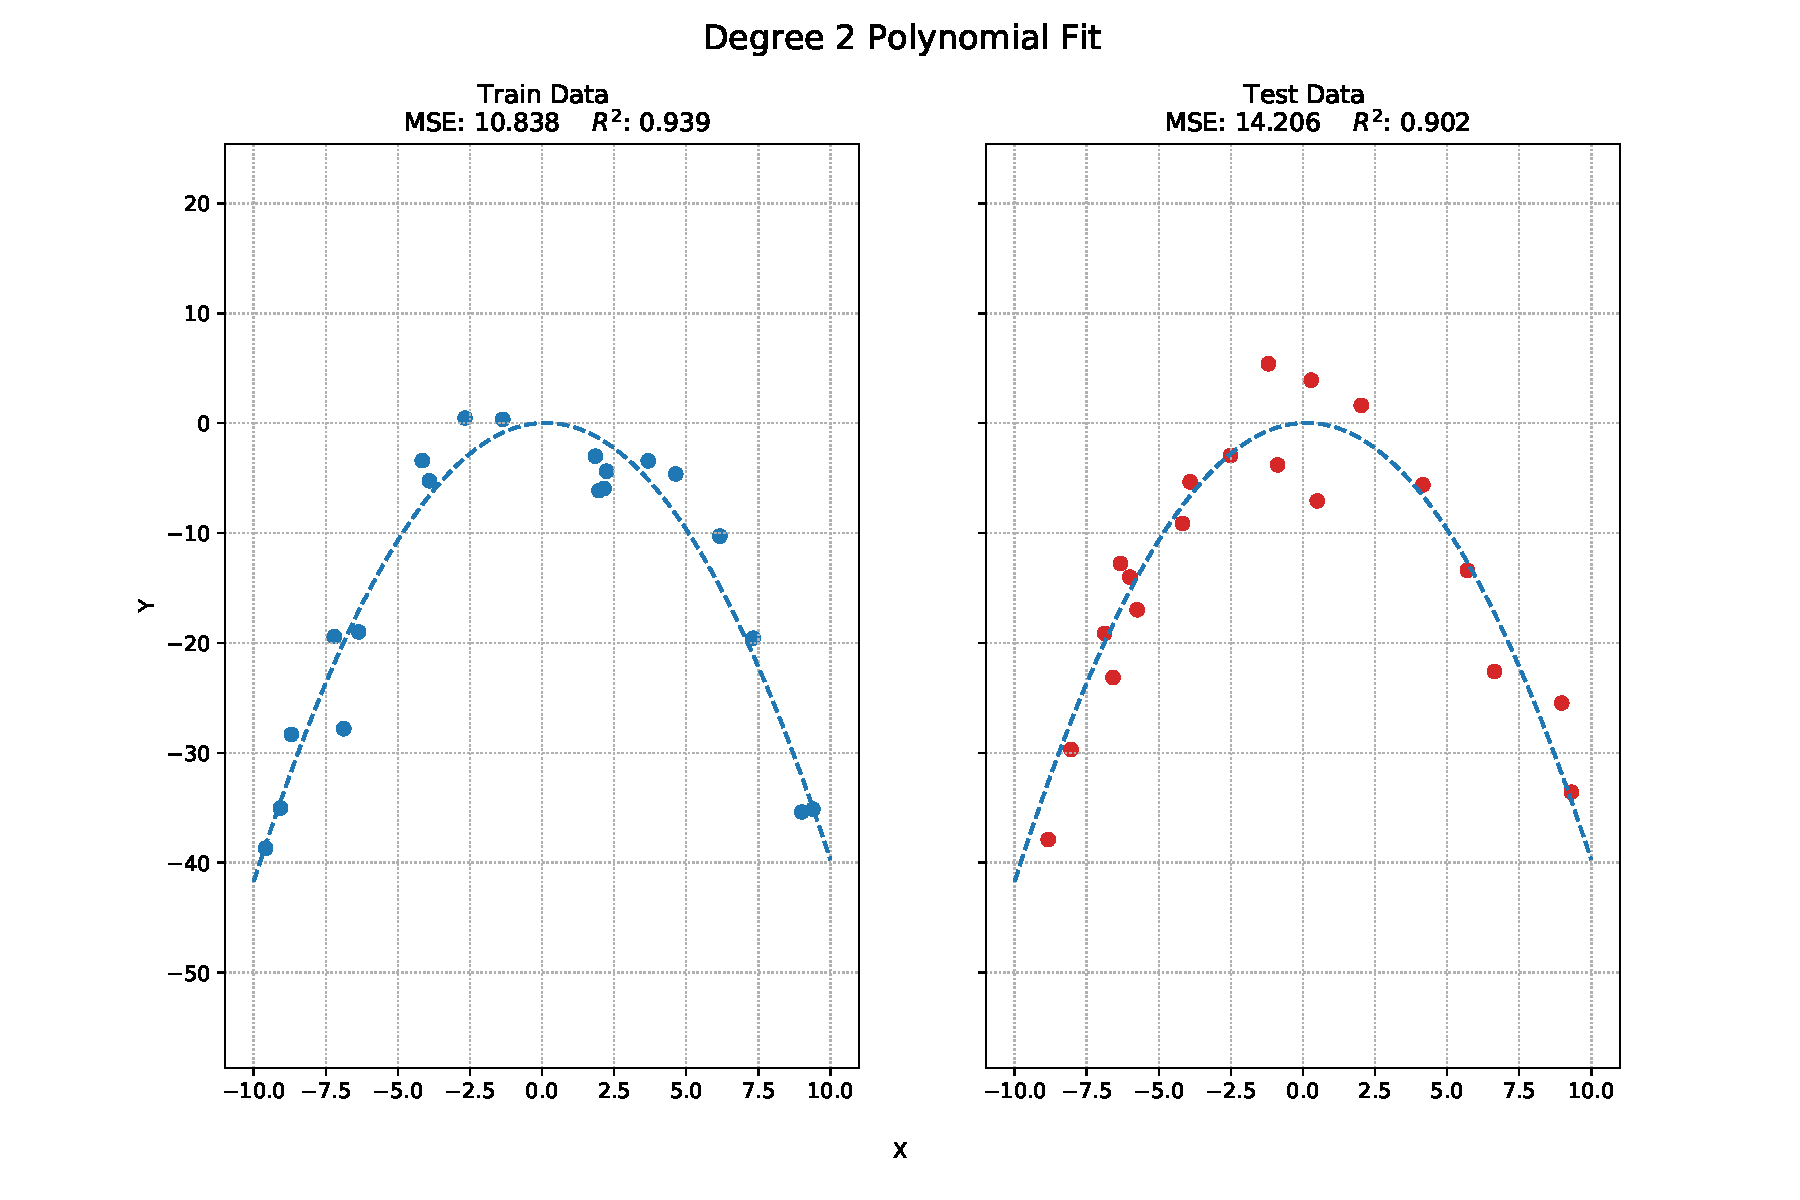
\includegraphics[width=0.5\textwidth]{figures/poly_fit_2.pdf}}
	\subfloat[]{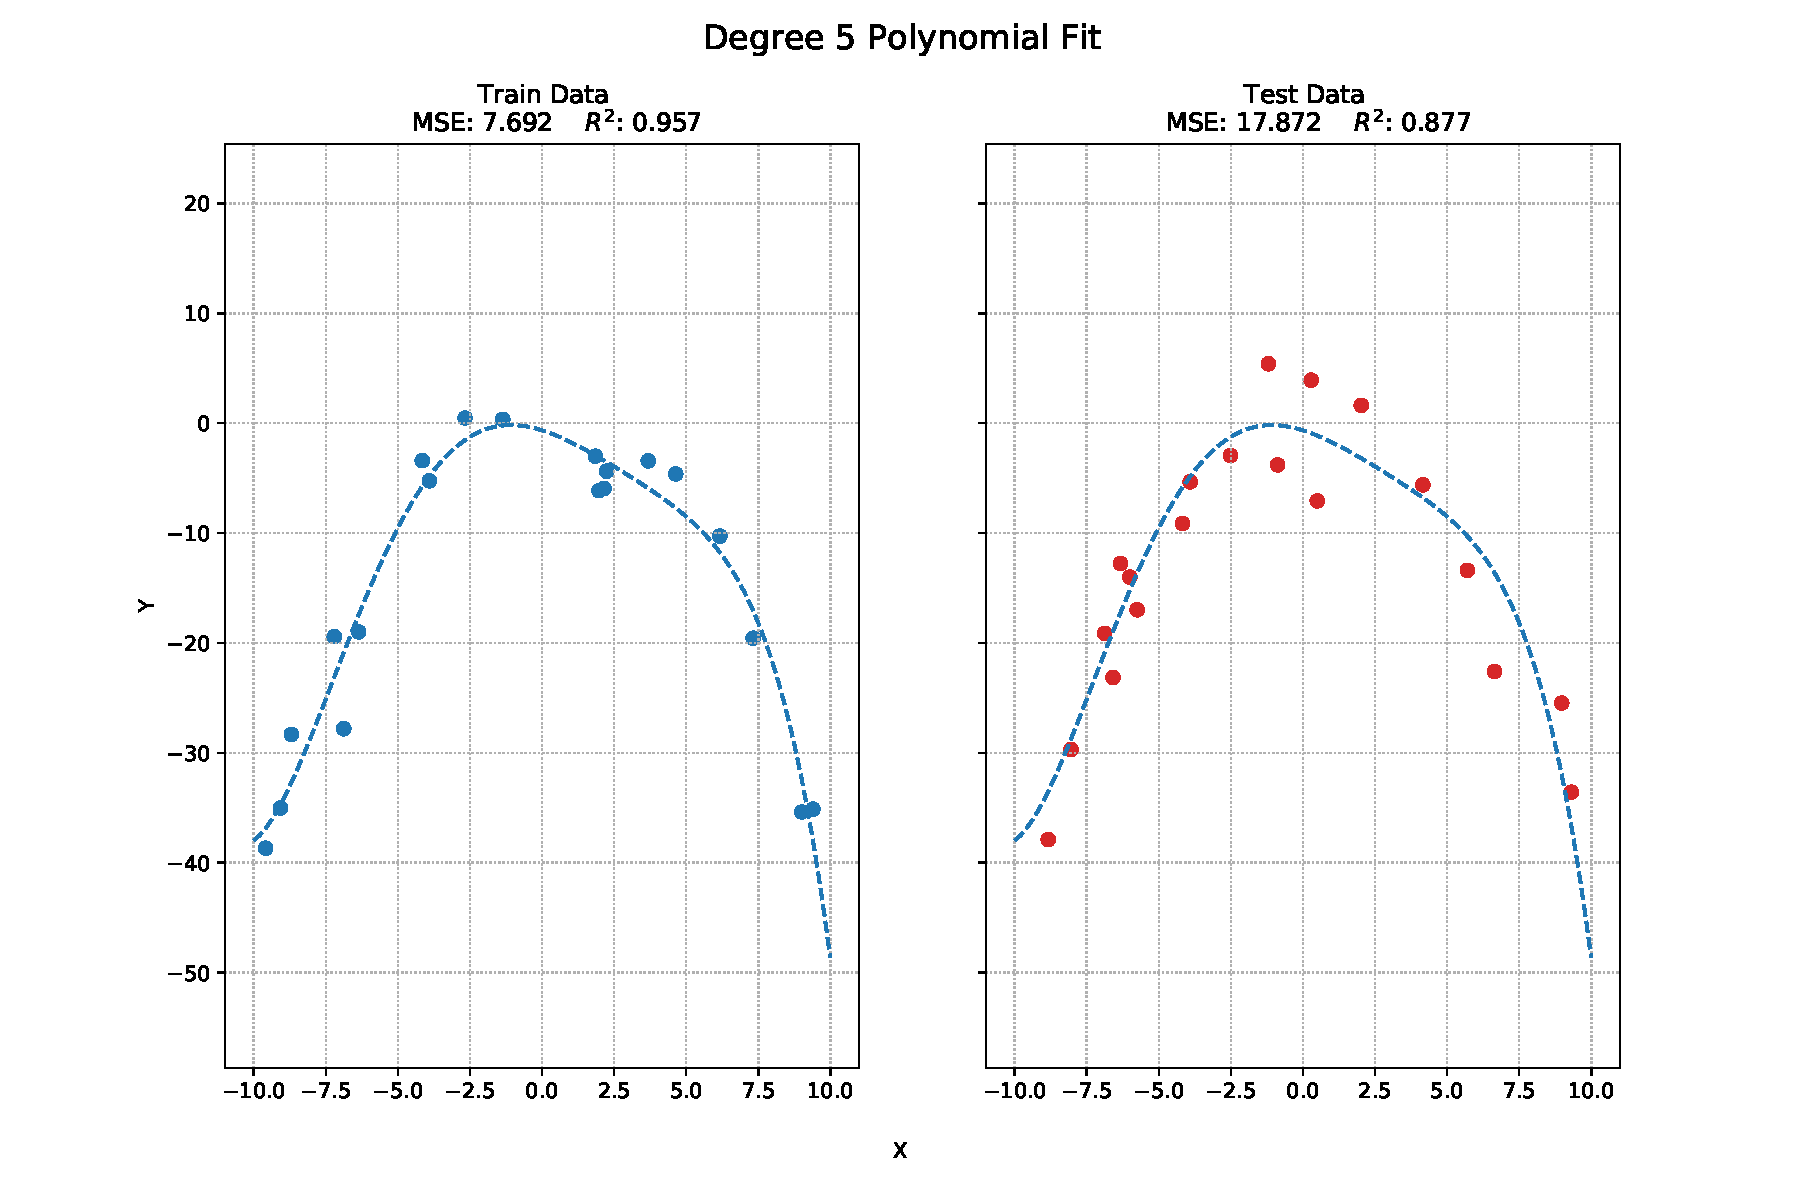
\includegraphics[width=0.5\textwidth]{figures/poly_fit_5.pdf}} \\
	\subfloat[]{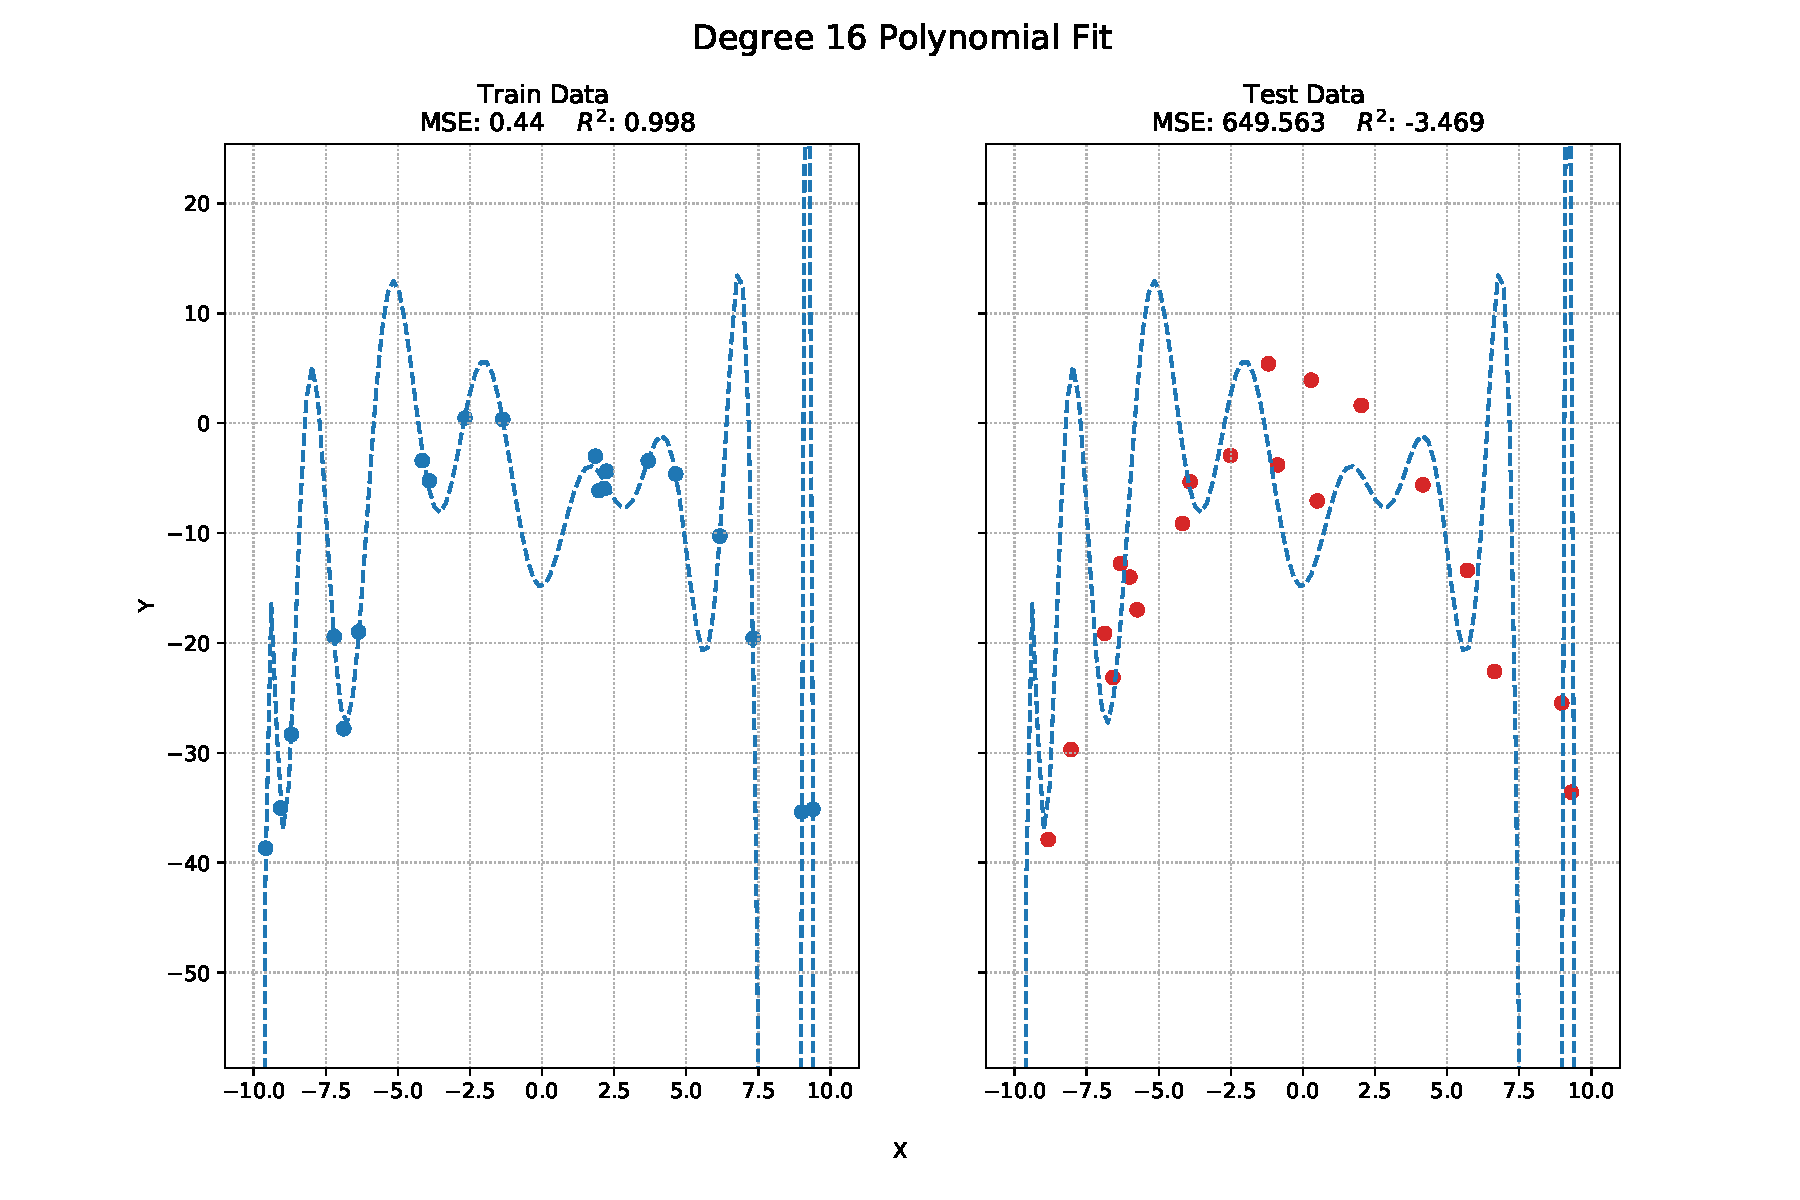
\includegraphics[width=0.5\textwidth]{figures/poly_fit_16.pdf}}
	\subfloat[]{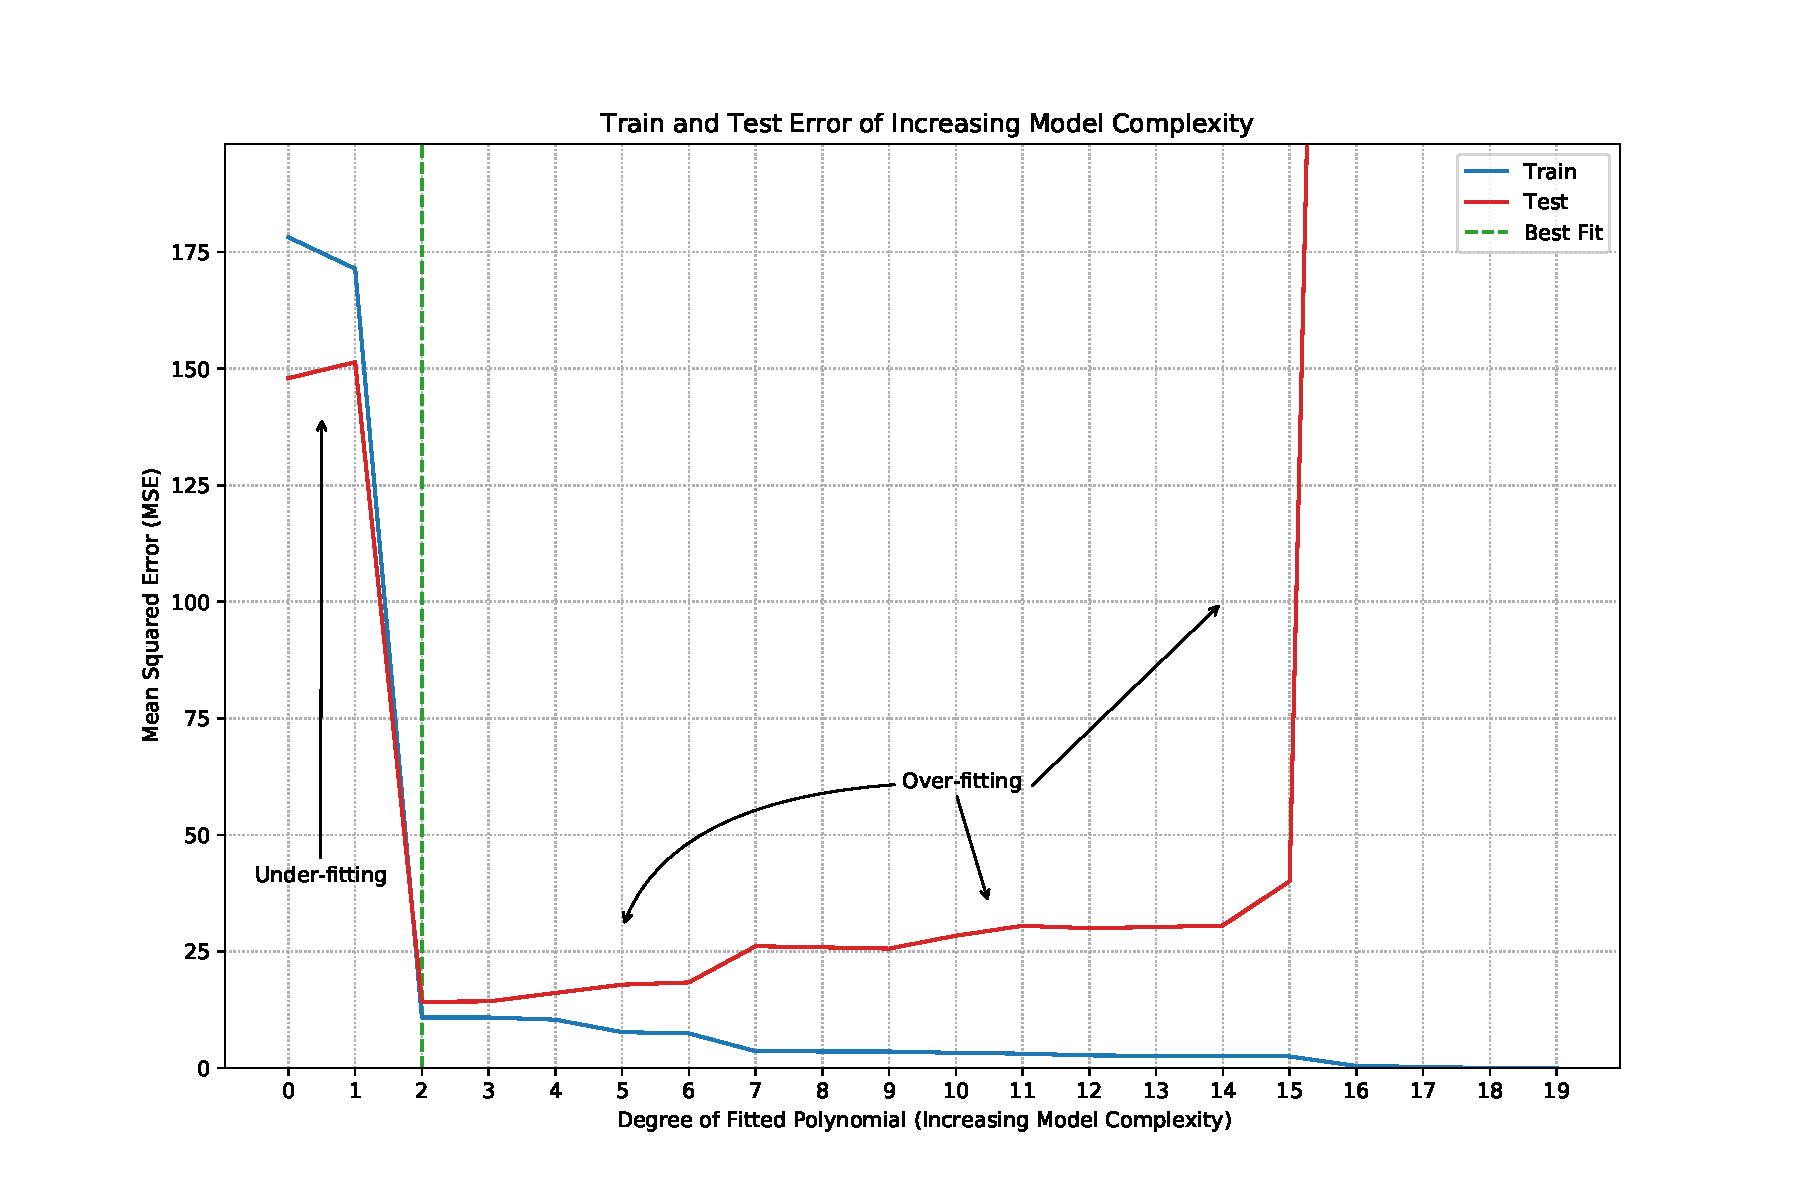
\includegraphics[width=0.5\textwidth]{figures/visualizing_overfitting.pdf}}
	\caption{Example of how increasing model complexity leads to better model fit on the train-set, but can come at the cost of increasingly worse performance on the test-set. Model fit here is measured visually and in terms of mean-squared-error (MSE: lower is better) and R-squared ($R^2$: closer to 1 is better). The dataset in (a) is generated by a degree-2 polynomial with some added noise and is split into train and test sets. A degree-1 polynomial underfits the data (b). More complex polynomials improve the fit on the train-set (c, d, e). However, increasingly complex polynomials become overfit as evidenced by increasingly worse test-set performance (d, e). The overall trend of increasing model complexity, how it relates to underfitting and overfitting, and where the tradeoff is optimal is captured in (f).}
	\label{fig:overfitting_example}
\end{figure}

The simplest way to approximate how well a model will perform on unseen data is to ``hold-out'' a portion of your dataset referred to as a \textit{test-set}, fit your model to the rest of the dataset referred to as the \textit{train-set}, and then check the fit and predictive performance of the model on the test-set. The objective is to create a model that has the best fit and predictive performance on the test-set rather than the train-set. If a model performs notably worse on the test-set, then you conclude the model is likely over-fit and you potentially reject it even though it may be the highest performing model on the train-set. This process is illustrated in Figure \ref{fig:overfitting_example}.  While this method is straightforward and generally effective it does have some drawbacks. The size of the train-set used to train the model is now smaller and may be too small to accurately reflect the model if it were trained on a larger dataset. The selection of which data is divided into the train and test sets may also bias the model and thus bias the estimate of its test-set evaluation. For example, if an essential group or cluster of similar data points are all put into the test-set then the models poor performance on the test-set could be misleading. Cross-validation is an attempt to alleviate these concerns and improve upon this method.

Cross-validation partitions the dataset randomly into K-many sets, with $2 \leq K \leq N$, where $N$ is the size of the dataset. It then uses one of the sets as the test-set, and combines the rest into the train-set. The model is fit on the train-set and then evaluated on the test-set. This process is then repeated using each of the K-many sets as the train and test splits and the average performance across all test-sets becomes the estimate for out-of-sample performance. In this way the entire dataset is used in both training and testing, helping to alleviate small data or biased train-test splitting concerns.

As you increase the value of K you also increase the size of the train-set which gives not only a better model fit but is more likely to over-fit if the model itself is prone to over-fitting, something we desire to find out. However, increasing the value of K also means you need to train and test the model more times. This is most noticeable when considering the extreme case where K is the size of the dataset, known as leave-one-out cross-validation (LOO-CV). In this case you train the model on all but one data point and then test on the one data point that was left out, and repeat for each data point. While this gives the best estimate of out of sample performance, it requires you to train the model a large number of times. In our modern big-data era, where datasets often number in the thousands or more, this can become computationally infeasible. A common way to deal with this is to reach a compromise by using a smaller value of K, usually 5 or 10.

While measuring the out-of-sample predictive performance of a model is of highest importance in evaluating a model, we have not discussed the specific measure itself. The example in Figure \ref{fig:overfitting_example} uses traditional measures of model fit based on point-predictions the models make, but Bayesian models produce entire distributions of estimates not just single point-predictions. Using a single point-prediction from an entire distribution greatly reduces and misses the vast majority of information that the entire distribution represents. Applied Bayesian statisticians have instead turned to the field of information theory to measure differences in distributions rather than point-estimates, and have tied these theories to the approximation of estimating LOO-CV performance without requiring refitting the model more times than is practical. We now discuss the development of these techniques as they are the primary way we evaluate models in this thesis.

Information theory is a field of mathematics concerned with representing data in a compact fashion (i.e. data compression) as well as transmitting data over a noisy channel and storing it in a way that is robust to errors \cite{Murphy2012}. Intuitively, quantifying information is viewed as measuring how much surprise there is in an event, where surprise relates to how likely or probable an event is. Thus, a surprising (lower probability) event is one that gives us more information than an unsurprising (higher probability) event. Claude Shannon first formalized these ideas in his foundational work on information theory \cite{Shannon1948} where he conceived of measuring information as the number of binary digits (bits) required to represent an event (or distribution). He extended this notion from discrete bits to a theoretical measure of a continuous amount of bits. In his work information is formally defined mathematically as information entropy:

\begin{equation}
H(p) = -Elog(p_i) = - \sum_{i=1}^{n} p_i log(p_i)
\end{equation}

where $p_i$ is the probability of event $i$ (or the i-th data point) occurring according to probability distribution $p$. In this way, information entropy can be thought of as measuring the uncertainty contained in a probability distribution as the average log-probability of the events (i.e. the data) \cite{McElreath2020}. We can then use this concept of information to reason mathematically about how much one probability distribution differs from another with respect to a dataset. Specifically, we can compute the average number of extra bits required to represent the data when using our models distribution as compared to the true distribution. This is captured mathematically in the form of Kullback-Leibler divergence (KL divergence) defined as:

\begin{equation}
D_{KL}(p,q) = \sum_{i} p_i (log(p_i) - log(q_i)) = \sum_{i} p_i log \left(\frac{p_i}{q_i} \right)
\end{equation}

The KL divergence can be thought of as the average difference in log probability between the true distribution (\textit{p}) and our models distribution (\textit{q}) \cite{McElreath2020}. It gives us a way to compare how similar two distributions are. Note that it does not satisfy some specific mathematical constraints, in particular it is generally not symmetric ($D_{KL}(p,q) \neq D_{KL}(q,p)$), which means KL divergence is not a ``measure'' or a ``distance'' in the strict mathematical sense. KL divergence instead represents how much effort is needed to turn one distribution into another, or how much one distribution diverges from another. It is useful because it gives us a rigorous way to compare how similar two distributions are; however, there is one glaring issue of practical significance. The issue is that we do not actually know what the true distribution is (\textit{p}) and therefore we are left with approximating the divergence. It turns out that the true distribution (\textit{p}) is not entirely necessary for comparing models because it is just an additive term which means you can compute the relative difference between models without actually knowing it \cite{McElreath2020}. Thus, we can use the sum of log probabilities of each observation known as the \textit{log-score}:

\begin{equation} \label{eq:log-score}
S(q) = \sum_i log(q_i)
\end{equation}

Relative differences in log-scores will match relative differences in KL divergence \cite{McElreath2020}. This means that we can compare models via their relative log-scores even though the magnitude of the log-score is not easily interpretable. In practice, for Bayesian modelling, we need to average over the posterior distribution (i.e. we need to consider the entire distribution of possible model parameters proportional to how likely they are) and compute a Bayesian log-score for a given dataset $y$ and model parameters $\theta_s$ known as the \textit{log-pointwise-predictive-density (lppd)}:

\begin{equation} \label{eq:lppd}
lppd(y, \theta) = \sum_i log \left( \frac{1}{S} \sum_s p(y_i | \theta_s) \right)
\end{equation}

The log-score has traditionally been scaled by -2 and referred to as the \textit{deviance}. This is because it has been shown that under general conditions and for many model types a difference between two deviances has a chi-squared distribution \cite{Dunn2018}. Thus, the factor of -2 would be there to scale the log-score to have this property to make more traditional computations such as likelihood ratio tests more convenient and interpretable. Modern users now tend to use just the log-score, or lppd, itself especially in a Bayesian context where traditional methods such as likelihood ratio tests are generally not used as often.

Thus we have derived a way of measuring statistical distance between a models distribution and the target distribution via information theory through the rigorously defined KL divergence. This statistical distance gives us a rigorous way of comparing models by evaluating which models distribution is closest to the target distribution. In practice we can not compute KL divergence precisely but instead approximate relative differences in KL divergence via the log-score, or equivalently the lppd in the Bayesian context. While the log-score is a way to measure the distance of our model from its target, it has the same flaw that nearly all methods for evaluating models have: \textit{the log-score will generally always improve as the model becomes more complex and thus has the potential to over-fit the dataset}. Researchers have developed a method of evaluation known as \textit{information criteria} which essentially adds a penalty term to the log-score in order to account for increasing model complexity. Thus, as increasingly complex models will generally have a better (higher) log-score, they will need to improve the log-score by more than the penalty otherwise it is likely they are fitting to random noise and not actually improving general model fit. This adjusted log-score can then be used to determine the best fitting model.

The first notable contribution to the development of information criterion was made by Japanese statistician Hirotugu Akaike \cite{Akaike1974}. The insight was that for each additional parameter added to a regression model, the test-set deviance becomes worse by a factor about twice the number of parameters. Akaike then showed that this is the case under some general conditions, and derived what he called \textit{an information criteria} which is now more commonly referred to as Akaike Information Criterion (AIC):

\begin{equation}
AIC = D_{train} + 2k \approx E(D_{test})
\end{equation}

where $D_{train}$ is the deviance on the train-set, $k$ is the number of parameters, and $E(D_{test})$ is the expectation of the deviance on the test-set. Sumio Watanade then generalized AIC to apply to a wider class of models and conditions to develop the Widely Applicable Information Criterion (WAIC) \cite{Watanabe2010}, sometimes referred to as Akaike Watanabe Information Criterion:

\begin{equation} \label{eq:waic}
WAIC(y, \theta) = -2 \left( lppd - \sum_i var_{\theta}(logp(y_i|\theta)) \right)
\end{equation}

where $y$ is the dataset and $\theta$ are the parameters of the model we are evaluating. The $lppd$ is the same as defined in equation \ref{eq:lppd}, and $\sum_i var_{\theta}(logp(y_i|\theta))$ is the penalty term which is an estimate of the sum of the variances of the log-likelihood for each observation ($i$) in the dataset. The penalty term is computed by computing the log-likelihood for each sample of parameters from the posterior distribution for the same observation $y_i$ and computing the variance of these log-likelihoods; then repeating this variance computation for each observation $y_i$ in the dataset and summing to yield the penalty term. The -2 transforms the lppd into a deviance measure as deviance was used for AIC rather than log-score. The negative sign before the 2 turns the lppd into a positive measure that we wish to minimize instead of maximize, and then the penalty term is a positive value that a more complex model needs to ``overcome'' in order to justify its use.

The WAIC provides a method for estimating the relative KL divergence by estimating the out-of-sample deviance by computing the negative lppd and adding a generalized penalty term that will make the estimate worse (larger) the more complex the model is. WAIC and information criterion in general attempt to estimate the out-of-sample deviance. More recent work attempts to bridge the gap between out-of-sample deviance and cross-validation resulting in the current state of the art method for estimating out-of-sample predictive fit that we use for model evaluation in this thesis.

Vethari et al. \cite{Vehtari2016} introduced an efficient computation for estimating LOO-CV from MCMC samples without requiring the repeated re-fitting of the model, referred to as Pareto-Smoothed Importance-Sampling Leave-One-Out cross-validation (PSIS-LOO). Their method also computes the lppd, but instead of adjusting it with the penalty term as in \ref{eq:waic}, they use importance sampling to re-weight the log-score of the lppd to more accurately reflect what the log-score for each data point would have been if that point had not been used to fit the model, hence the estimation of LOO-CV by re-weighting rather than re-fitting the model. The insight of Vehtari et al. is that the weights needed in order to re-weight the posterior samples for a given data point (e.g. the weights $w_s$ for re-weighting data point $y_1$: $\frac{1}{\sum_s w_s} \sum_s w_s p(y_1 | \theta_s)$) in a manner that resembles what the probability would have been if that data point had not actually been observed in the dataset the model was trained on, turn out to be the inverse of the probability that the posterior draw gave to the held out data point (e.g. the weights for $y_1$ are $w_s = \frac{1}{p(y_1|\theta_s)}$). Vehtari et al. further improved the stability of the importance sampling estimates by showing the upper tail of these importance weights fit a generalized Pareto distribution. Instead of using the estimated importance weights themselves, they instead use the weights to fit a generalized Pareto distribution and then use the weights implied by the fitted Pareto distribution resulting in Pareto-smoothed weights. PSIS-LOO is thusly computed as:

\begin{equation} \label{eq:psis-loo}
PSIS-LOO(y, \theta) = \sum_i log \left( \frac{1}{\sum_s w_s^i} \sum_s w_s^i p(y_i | \theta_s) \right)
\end{equation}

where $w_s^i$ is the Pareto-smoothed importance weight for data point $y_i$ with sampled parameters $\theta_s$. The rest is the same as in \ref{eq:lppd} with the key change being the re-weighting performed by multiplying by the weights ($w_s^i$) and re-averaging proportional to the re-weighting ($\sum_s w_s^i$).

The PSIS-LOO estimate is also an estimate of the out-of-sample relative KL divergence. As a result, the PSIS-LOO estimates are often similar to WAIC estimates in practice, but were shown to be more stable and consistent than WAIC estimates \cite{Vehtari2016}. The models that are fit and compared in this thesis all gave near identical results for both PSIS-LOO and WAIC. We have chosen to use just PSIS-LOO as it has become the modern standard.

\subsection{Posterior Predictive Checks} \label{ppc}

Posterior predictive checks (PPCs) give us a way to visually check how well a model fits the dataset. Since Bayesian models are generative, we can use the fitted model to simulate values and then observe how closely these generated values resemble the observed values of the dataset. If the distribution of simulated values closely resembles the observed dataset then we say that the model is ``well-specified'' or is a good fit to the dataset. If the distribution of simulated values does not closely resemble the observed dataset then we say that the model is ``misspecified'' or is a bad fit to the dataset. It is notable that PPCs do not only reveal that a model is potentially misspecified but often also give insight into how to potentially improve the model by visually seeing for which data points the model is struggling to fit well. In this way PPCs are not only useful for model evaluation but for model building as well. PPCs informed the models chosen in the second data experiment discussed in section \ref{experiment_2}.
